\documentclass[../../Problems]{subfiles}
\begin{document}
\subsection{Bernoulli's Triangle}{\label{pp:bernoullistriangle}}
You might have heard about \href{https://youtu.be/0iMtlus-afo}{Pascal's Triangle}. 
The $k$\textsuperscript{th} element of row $n$ of Bernoulli's Triangle is obtained by as shown in \ref{fig:bernoullistriangle} summing all elements of the row $n$ (row $0$ is the first row) until the $k$\textsuperscript{th} element (partial sums).
\begin{figure}[H]
	\centering
	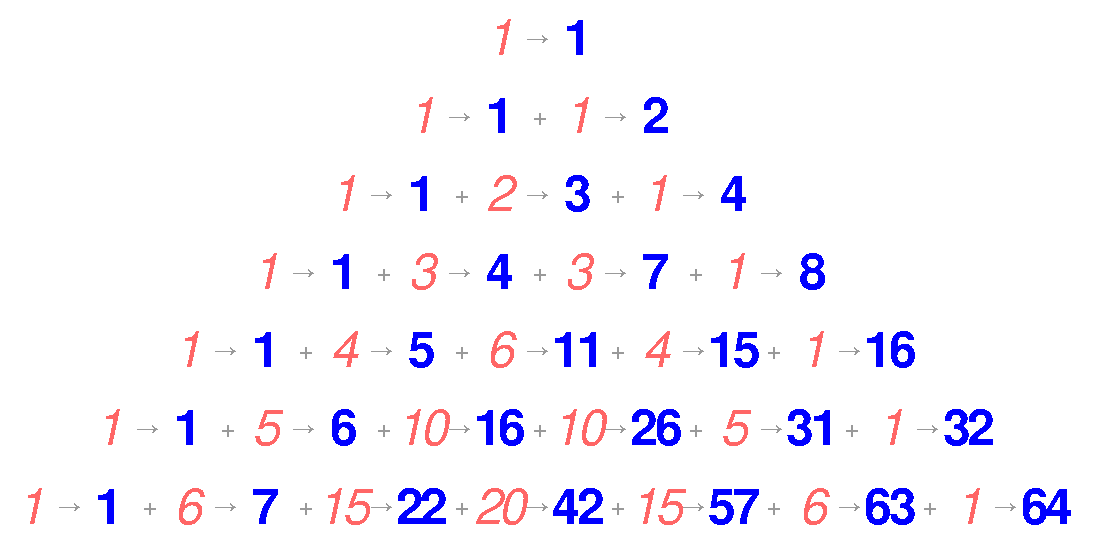
\includegraphics[width = 0.35\linewidth]{Bernoulli's Triangle.pdf}
	\caption{\textbf{\textcolor{blue}{Bernoulli's triangle}} from \textit{\textcolor{pink}{Pascal's triangle}} (\href{https://bit.ly/bernoullis-triangle}{Image} by \href{https://commons.wikimedia.org/wiki/User:Cmglee}{Cmglee} licensed under \href{https://creativecommons.org/licenses/by-sa/4.0/}{CC BY-SA 4.0})}
	% \caption{Bernoulli's triangle (\textbf{\textcolor{blue}{blue bold}} text) from Pascal's triangle (\textit{\textcolor{pink}{pink italics}}) (\href{https://bit.ly/bernoullis-triangle}{Image} by \href{https://commons.wikimedia.org/wiki/User:Cmglee}{Cmglee} licensed under \href{https://creativecommons.org/licenses/by-sa/4.0/}{CC BY-SA 4.0})}
	\label{fig:bernoullistriangle}
\end{figure}
% Formally given as below
% \begin{equation}
% B_{n,k} =  \sum _{p=0}^{k}{n \choose p}
% \end{equation}
\vspace{-1.5em}
\textbf{Problem Statement:}\\
Print the left-aligned Bernoulli's Triangle for all given $n$. See Starter code (below) for more details.
\begin{testcases}
	{$t$ \hfill(number of test cases, an integer)\\$n_1\ n_2\ \ldots\ n_t$ \hfill($t$ space seperated integers for each testcase)}
	{Bernoulli's Triangle \hfill(left-aligned, each test case on a newline)}
	{$0 \leq n_i \leq 20$}
	{4\\0 1 2 10}
	{1\\[1em]1\\1 2\\[1em]1\\1 2\\1 3 4\\[1em]1\\1 2\\1 3 4\\1 4 7 8\\1 5 11 15 16\\1 6 16 26 31 32\\1 7 22 42 57 63 64\\1 8 29 64 99 120 127 128\\1 9 37 93 163 219 247 255 256\\1 10 46 130 256 382 466 502 511 512\\1 11 56 176 386 638 848 968 1013 1023 1024}
	{https://github.com/paramrathour/CS-101/tree/main/Starter Codes/Bernoulli's Triangle.cpp}
\end{testcases}
\begin{funvideo}
\href{https://youtu.be/0iMtlus-afo}{Pascal's Triangle -- Numberphile}\\
\href{https://youtu.be/J0I1NuxUcpQ}{What You Don't Know About Pascal's Triangle -- Tipping Point Math}
\end{funvideo}
\end{document}